\documentclass[tikz,border=2pt]{standalone}
\usepackage{pgfplots}
\pgfplotsset{compat=1.18}

\begin{document}
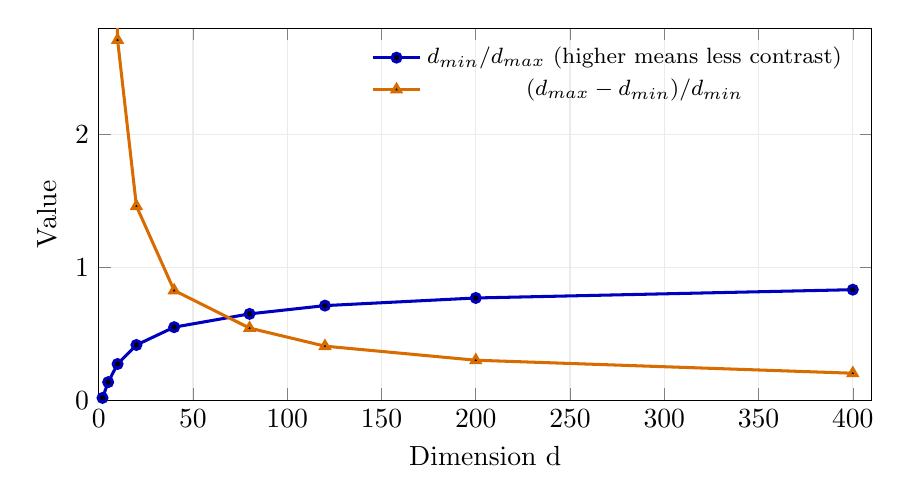
\begin{tikzpicture}
\begin{axis}[
  width=0.94\textwidth,
  height=0.52\textwidth,
  xlabel={Dimension d},
  ylabel={Value},
  xmin=0, xmax=410,
  ymin=0, ymax=2.8,
  legend style={at={(0.98,0.98)},anchor=north east,draw=none,fill=none,font=\footnotesize},
  grid=major,
  major grid style={draw=black!8},
]
\addplot[draw=blue!75!black, line width=1.1pt, mark=*, mark size=1.6pt] coordinates {(2.00000,0.01695) (5.00000,0.13567) (10.00000,0.27219) (20.00000,0.41526) (40.00000,0.54948) (80.00000,0.64954) (120.00000,0.71182) (200.00000,0.76924) (400.00000,0.83172)};
\addlegendentry{$d_{min}/d_{max}$ (higher means less contrast)}
\addplot[draw=orange!85!black, line width=1.1pt, mark=triangle*, mark size=1.7pt] coordinates {(2.00000,78.18493) (5.00000,7.07837) (10.00000,2.71170) (20.00000,1.46059) (40.00000,0.82600) (80.00000,0.54264) (120.00000,0.40660) (200.00000,0.30079) (400.00000,0.20274)};
\addlegendentry{$(d_{max}-d_{min})/d_{min}$}
\end{axis}
\end{tikzpicture}
\end{document}
